\documentclass[sigconf,nonacm,anonymous]{acmart}

\usepackage{tabularx, booktabs}
\usepackage{ragged2e}
\newcolumntype{L}{>{\RaggedRight\arraybackslash}X}
\usepackage[utf8]{inputenc}
\usepackage[T1]{fontenc}
\usepackage{tcolorbox}
\usepackage{amsmath, amssymb} 
\usepackage{parskip}
\usepackage{graphicx}
\usepackage{longtable}
\usepackage[svgnames]{xcolor}
\usepackage{hyperref}
\usepackage{footnote}
\usepackage{todonotes} % Added to support the \todo{} command in your text
\usepackage{amsthm}

\newcommand\vldbdoi{XX.XX/XXX.XX}
\newcommand\vldbpages{XXX-XXX}
\newcommand\vldbvolume{14}
\newcommand\vldbissue{1}
\newcommand\vldbyear{2020}
\newcommand\vldbauthors{\authors}
\newcommand\vldbtitle{\shorttitle}
\newcommand\vldbavailabilityurl{URL_TO_YOUR_ARTIFACTS}
\newcommand\vldbpagestyle{plain}

\newtheorem{example}{Example}
\newtheorem{problem}{Problem}

\newtcolorbox{examplebox}{
  colback=blue!10,
  colframe=blue!20,
  arc=2mm,
  fonttitle=\bfseries,
  boxrule=0mm,
  boxsep=1mm,
  left=0mm,
  right=0mm,
  top=0mm,
  bottom=0mm
}

\newtcolorbox{pbox}{
  colback=black!5,
  colframe=black!30,
  arc=2mm,
  fonttitle=\bfseries,
  boxrule=0mm,
  boxsep=1mm,
  left=0mm,
  right=0mm,
  top=0mm,
  bottom=0mm
}

\newtcolorbox{defbox}{
  colback=white,
  colframe=black!100,
  arc=1mm,
  fonttitle=\bfseries,
  sharp corners=all,
  boxrule=0.2mm,
  boxsep=1mm,
  left=0mm,
  right=0mm,
  top=0mm,
  bottom=0mm
}

\begin{document}
\title{A Modular Framework for LLM-Guided Pattern Analysis}

%%
%% The "author" command and its associated commands are used to define the authors and their affiliations.
\author{Ben Trovato}
\affiliation{%
  \institution{Institute for Clarity in Documentation}
  \streetaddress{P.O. Box 1212}
  \city{Dublin}
  \state{Ireland}
  \postcode{43017-6221}
}
\email{trovato@corporation.com}

%%
%% The abstract is a short summary of the work to be presented in the
%% article.
\begin{abstract}
Exploratory pattern analysis is difficult not simply because data are large, but because end-to-end analytical workflows require coordinated, strategic reasoning over textual and tabular data alike. In this work, we present a modular framework for LLM-assisted pattern analysis. Our framework formulates inputs to language models in the forms of triples containing (a) mathematical definitions, (b) corresponding textual interpretation, and (c) a set of example pairs gluing textual and tabular evidence. Based on these, we map users from partially specified pattern components to target components, thus enabling pattern recognition, formulation, as well as instance discovery to be expressed within a unified formal representation. 

We investigate whether such complementary representations of pattern knowledge, including examples, textual descriptions, formal definitions, and their combinations, improve LLM-guided exploration in an end-to-end, analyst-like workflow environment. We instantiate the approach through a suite of prompting strategies and evaluate our proof-of-concept over the USPTO dataset and its corresponding WIPO report corpus. Our results validate that modular, component-wise grounding can help make LLM reasoning more coherent in exploratory pattern analysis, while also highlighting the current limits of LLMs for the same.
\end{abstract}

\maketitle

%%% do not modify the following VLDB block %%
%%% VLDB block start %%%
\pagestyle{\vldbpagestyle}
\begingroup\small\noindent\raggedright\textbf{PVLDB Reference Format:}\\
\vldbauthors. \vldbtitle. PVLDB, \vldbvolume(\vldbissue): \vldbpages, \vldbyear.\\
\href{https://doi.org/\vldbdoi}{doi:\vldbdoi}
\endgroup
\begingroup
\renewcommand\thefootnote{}\footnote{\noindent
This work is licensed under the Creative Commons BY-NC-ND 4.0 International License. Visit \url{https://creativecommons.org/licenses/by-nc-nd/4.0/} to view a copy of this license. For any use beyond those covered by this license, obtain permission by emailing \href{mailto:info@vldb.org}{info@vldb.org}. Copyright is held by the owner/author(s). Publication rights licensed to the VLDB Endowment. \\
\raggedright Proceedings of the VLDB Endowment, Vol. \vldbvolume, No. \vldbissue\ %
ISSN 2150-8097. \\
\href{https://doi.org/\vldbdoi}{doi:\vldbdoi} \\
}\addtocounter{footnote}{-1}\endgroup
%%% VLDB block end %%%

%%% do not modify the following VLDB block %%
%%% VLDB block start %%%
\ifdefempty{\vldbavailabilityurl}{}{
\vspace{.3cm}
\begingroup\small\noindent\raggedright\textbf{PVLDB Artifact Availability:}\\
The source code, data, and/or other artifacts have been made available at \url{\vldbavailabilityurl}.
\endgroup
}
%%% VLDB block end %%%

\section{Introduction}

Pattern analysis using large language models (LLMs) is challenging not only because data are large, but because meaningful patterns must often be articulated before they can be searched, compared, or validated. For non-experts, the barrier may be partially technical and partly conceptual: even when an interesting phenomenon is visible, it may not be intuitive how to formalize that observation or tie it across multiple sources of evidence. Recent advancements in language model capabilities have created new opportunities to lower this barrier by supporting more natural interaction with data. However, as the complexity associated with underlying tasks increases, purely linguistic prompting can become insufficient for preserving the logical and mathematical discipline that complex pattern analysis necessitates.

Our problem is inherently evident in exploratory workflows that comprise a mixture of structured and unstructured data. For example, a textual report may describe an interesting pattern - for instance, a major turning point, convergence across trends, or association rules - while the corresponding evidence may live in structured counts or time series. In order to facilitate powerful human-AI workflows, LLM-powered agents must therefore do more than answer questions fluently: they must \textit{recognize} cross-modal evidence, \textit{formulate the mathematical logic} of a pattern, and further use that logic to \textit{search for insights} in an integrated manner.

In this paper, we address this problem by proposing a modular framework for LLM-assisted pattern analysis. To this light, we represent a pattern in the form of pattern triple $\mathcal{P} = (\mathcal{M}, \mathcal{T}, \mathcal{E})$ as a composition of  mathematical definition ($\mathcal{M}$), its textual interpretation ($\mathcal{T}$) and examples ($\mathcal{E}$). By formulating analysis as a mapping from partially known components to desired components, our proposed framework leverages the concept of component-wise grounding: the model resolves one analytical element at a time instead of collapsing the objective into a single hop. This design is intended to both reduce contextual drift and keep reasoning anchored to the available evidence.

\begin{figure*}[t]
\centering
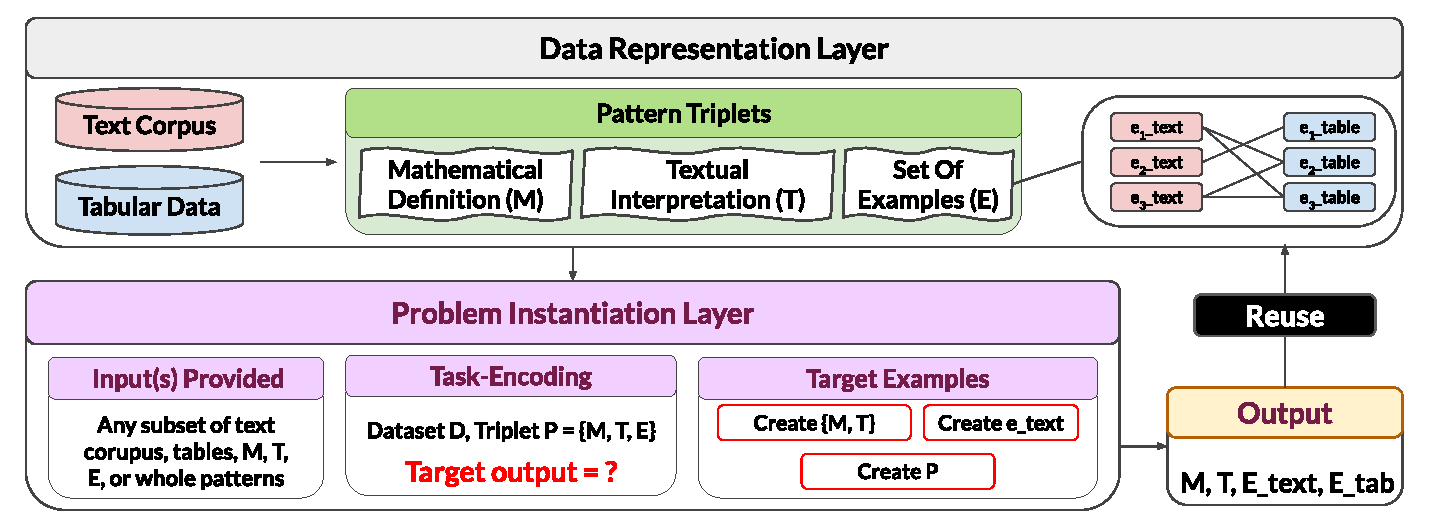
\includegraphics[width=114mm]{alnkrit.eps}
\caption{Overview Of Our Framework}
\label{fig:framewokr}
\end{figure*}

The core focus of our work is to investigate the aforesaid design principle in contrast to claiming a general-purpose discovery engine. Our focus is to test whether complementary representations of pattern knowledge - including examples, textual descriptions, formal definitions, as well as their combinations - materially improve an LLM's ability to recognize, formalize, and operationalize patterns in an end-to-end exploratory workflow. In this paper, we investigate and test our hypothesis through a USPTO case study using structured, tabular data and a corresponding WIPO report corpus. Our key contributions include:

\begin{itemize}[leftmargin=0pt]
\item We re-imagine and formalize the pattern-analysis workflows as transformations over multiple key modular pattern components.
\item We propose a framework that supports component-wise grounding through mathematical definitions, textual descriptions, and example pairs.
\item We perform an extensive performance evaluation study on the USPTO and WIPO datasets demonstrating how different pattern representations affect LLM-guided exploration in practice.
\end{itemize}

\textcolor{red}{Raghav: describe Figure~\ref{fig:framewokr} once doctor chengkai li approves of it.}

\begin{figure*}[t]
\centering
\includegraphics[width=\textwidth]{PatternCards.pdf}
\caption{Pattern cards illustrating the components of a pattern. Each card contains a mathematical definition, a textual description, and example pairs consisting of textual and tabular examples.}
\label{fig:pattern-cards}
\end{figure*}

\section{Related Works}
In the context of relevant literature, this Section highlights prior efforts that focus on (a) fine-tuning task instructions, (b) in-context example selection for downstream performance optimization, and (c) benchmarks that expose the need for \textit{explicit} decomposition.
\subsection{Instruction Tuning and Task Descriptions}

\cite{weller-etal-2020-learning} early demonstration that models can generalize to unseen tasks when natural-language task descriptions are treated as first-class supervision

\cite{mishra-etal-2022-cross} showed that diverse human-written instructions can induce broad transfer across tasks

\cite{wei2021finetuned} established instruction tuning as a scalable recipe for zero-shot generalization, making instruction format a central design variable rather than an afterthought

\cite{sanh2021multitask} cast many tasks into a prompted text-to-text format and showed that multitask prompting can improve cross-task generalization without task-specific architectures

\cite{wang-etal-2022-super} expanded the instruction-tuning paradigm to a large and heterogeneous benchmark, providing a strong empirical basis for studying instruction robustness

\cite{wang-etal-2023-self-instruct} showed that instruction-following behavior can be bootstrapped from model-generated tasks and responses, underscoring the importance of instruction diversity

\cite{honovich-etal-2023-instruction} inverted the problem by asking models to infer task descriptions from examples, which is directly relevant to our concern with representational abstractions

\subsection{In-Context Learning and Example Selection}

\cite{nipsxyz} made few-shot prompting a mainstream paradigm by showing that large language models can adapt to tasks from examples alone

\cite{lu-etal-2022-fantastically} demonstrated that example order can strongly affect performance, highlighting the fragility of naive demonstration design

\cite{min-etal-2022-rethinking} argued that label-space and input-format regularities explain more of in-context learning than previously assumed

\cite{rubin-etal-2022-learning} treated prompt selection as a retrieval problem, suggesting principled ways to choose representative examples

\cite{nipsabc} connected in-context behavior to the statistical structure of pretraining data

\cite{nipsabcxyz} offered a controlled theoretical perspective on the algorithmic limits of in-context learners

\cite{xie2022an} provided a mechanistic explanation of in-context learning, which is useful when interpreting why some pattern representations transfer better than others

\subsection{Benchmarks for Decomposed and Multi-Step Reasoning}

\cite{yang-etal-2018-hotpotqa} made multi-hop reasoning and supporting-fact identification central to question answering evaluation

\cite{ho-etal-2020-constructing} constructed questions with explicit reasoning-step coverage, reducing shortcuts and exposing genuine multi-hop difficulty

\cite{ferguson-etal-2020-iirc} focused on incomplete-information reading comprehension, where answering requires seeking additional context beyond the initial passage

\cite{wolfson-etal-2020-break} benchmarked question decomposition itself, treating the generation of subquestions as a core capability

\cite{geva-etal-2021-aristotle} targeted questions whose reasoning strategy is implicit rather than stated, an especially relevant challenge for open-ended analytical discovery

\cite{talmor2021multimodalqa} required reasoning across text, tables, and images, broadening decomposition beyond single-modality evidence paths

\cite{trivedi-etal-2022-musique} systematically composed single-hop questions into genuine multihop problems, offering a clean benchmark for connected reasoning

\section{Framework}
\label{sec:framework}

The goal of this framework is to formulate analytical tasks by modularizing \textit{patterns} and \textit{data} into components. These components act as building blocks that allow analytical problems to be expressed in a structured format to the computational tools.

Instead of defining broad research goals, the framework encourages users to
express analytical tasks as mappings between patterns as \textbf{Inputs} and \textbf{Outputs}.
Users take the information currently available, such as mathematical definitions of multiple patterns, examples of a single pattern, etc., and define it as the input to a tool. They then specify a desired output, which may represent new knowledge that is not currently available to them. The transformation from input to output is performed by the LLM. The input–output formulation allows users to clearly state what information is given to the tool and what result they expect in return.

\begin{table*}[t]
\centering
\small
\setlength{\tabcolsep}{4pt}
\renewcommand{\arraystretch}{1.7} % Space for nested sets/pairs
\caption{Representative problem formulations and signatures grounded in the USPTO study.}
\label{tab:problem-catalog}
\begin{tabular}{c|p{0.26\textwidth}|p{0.30\textwidth}|p{0.34\textwidth}}
\hline
\textbf{ID} & \textbf{Formulation} & \textbf{Description} & \textbf{Definition} \\
\hline

1 & 
$D: (\_, D_{tabular})$ \newline
$P_1 : (?, T_1, \_)$
& Utilizing only $T_1$ from the convergence/divergence pattern, formulate $M_1$ that is suitable for $D_{tabular}$
& Utilize text description of a pattern to formulate its mathematical definition, that is suitable for the provided tabular dataset \\

2 & 
$D: (D.text, \_)$ \newline
$P_1 : (M_1, T_1, \{(?, \_)\})$
& \textbf Utilizing only $M_1$ and $T_1$ from the convergence/divergence pattern, we find $E1.text$ within $D.text$ for the same.
& Utilize the Mathematical definition and Text Description of a pattern to find text examples for the same pattern in reports. \\

3 & 
$D: (\_, D_{tabular})$ \newline
$P_1 : (\_, \_, \{(E_{1,text}, ?)\})$
& \textbf Utilizing only $E1.text$ from the convergence/divergence pattern, we find $E_{1_{tabular}}$ within $D_{tabular}$ for the same.
&  Utilizing an observed textual example of a pattern, locate the corresponding tabular example within tabular data\\

4 &
$D: (D.text, D_{tabular})$ \newline
$P_1 : (M_1, T_1, \_)$ \newline
$P_2 : (?, ?, \_)$
& Utilize $M_1$ and $T_1$ from the convergence/divergence pattern to synthesize $M_2$ and $T_2$ for a new pattern, namely, the change-point pattern
& Utilize Math definition and text description of a known pattern as reference to synthesize the math definition and text description of a new pattern that is aligned with text and tabular data \\

5 & 
$D: (\_, \_)$ \newline
$P_1 : (M_1, T_1, \_)$ \newline
$P_2 : (?, T_2, \_)$
& Utilize the $M_1$ and $T_1$ from the convergence/divergence pattern and $T_2$ from change-point pattern as reference, to synthesize $M_2$ for the change-point pattern
& Formulate the mathematical definition of pattern by utilizing its text description along with the math definition and text description of a new pattern as reference \\

6 & 
$D: (\_, \_)$ \newline
$P_1 : (?, ?, \{(E1.text, E1.tab)\})$
& Utilizing E1.text, and E1.tab formulate M1 and T1 for the convergence/divergence pattern.
& Utilizing one example pair for a pattern, formulate its mathematical definition and text description\\

7 & 
$D: (D.text, D_{tabular})$ \newline
$P_1 : (\_, \_, \{(E1.text, E1.tab),(?,?)[2] \})$
& Utilizing E1.text and E1.tab as basis, to mine other examples of convergence/divergence pattern from $D.text$ and $D_{tabular}$ 
& Utilize a given example pair to mine two other example pairs for the same pattern from tabular data and text reports\\

8 & 
$D: (D.text, D.tab)$ \newline
$P_1 : (M1, \_, \{(?,?)[2] \})$
& Utilize M1 to find two example pairs from $D.text$ and $D.tab$ for the convergence/divergence pattern
& Utilize the mathematical definition of a pattern to mine two examples from text reports and tabular data.\\

\hline
\end{tabular}
\end{table*}

\subsection{Pattern and Data Representation}

The framework operates on patterns as primary objects of analysis, with data providing the source from which patterns are identified and the context in which they are grounded.

This framework works with two types of data: \textbf{tabular data} ($D.tab$) and \textbf{textual data} ($D.text$). Tabular data refers to structured datasets such as spreadsheets or relational tables. Textual data refers to information expressed in natural language, such as patent landscape reports, corporate reports, or technical documents. For the purpose of this study, tabular data corresponds to a \textbf{single unified table}, and reports correspond to a \textbf{set of textual reports}.

A Pattern is defined as a recurring structural behavior found in data. For instance, in the context of multiple time-series datasets, one can observe periods where the gap between series either closes (convergence) or widens (divergence). The behavior portrayed by data during these periods can be called a convergence or divergence pattern. Similarly, all such observable structural behaviors, where data follows a recognizable and repeatable logic, we specify them as patterns.

To facilitate analysis, a pattern is modularized into these components: a Mathematical Definition ($M$), a Textual Description ($T$), and a set of Examples ($E$).

\textbf{Examples} ($E$) is a set comprised of pairs.
Pairs are denoted by $e$, making $E = \{e_1, e_2, ...\}$. 
Each pair ($e$) is composed of two parts: a \textbf{Tabular Example} 
($E.tab$) and a \textbf{Textual Example} ($E.text$).

Textual Example of a pattern is an observed instance that is found in text data, such as reports. A textual example for the 
convergence/divergence pattern is shown in Figure~\ref{fig:pattern-cards} 
($E1.text$). The textual example ($E1.text$) for the convergence/divergence pattern describes two time series, the patent count for the GAN family and the patent count for LLM/diffusion models. It notes that one is growing much faster than the other.\todo{Provide URLs to report and data.}

Corresponding to the textual example ($E.text$), there exists a tabular example ($E.tab$) found in tabular data. For the convergence/divergence pattern, $E1.tab$ is the corresponding tabular example for the textual example $E1.text$

Since, these two correspond to the same instance of a pattern in different modalities, together, ($E1.text$, $E1.tab$) form a pair. Although examples are represented as pairs, textual and tabular examples may also exist independently. In practice, only one form of example may be available for a pattern. The framework therefore allows analytical tasks to be formulated using either $E.text$ or $E.tab$ alone. The pair representation simply preserves the correspondence between the two forms when both are available.\todo{improve figure resolution.}

The behavior illustrated by the examples can be summarized using a 
\textbf{textual description} ($T$). A textual description explains the 
common behavior shared by the examples using natural language. In the 
pattern card, the behavior observed in the example pair ($E1.text$, $E1.tab$) is 
described by the textual description $T_1$ in 
Figure~\ref{fig:pattern-cards}. Unlike examples which is a set, a pattern has a single textual description that summarizes 
its behavior.

%\textcolor{red}{Raghav: Should we also add negative examples in the prompt and see if we get better answers? Should be interesting. \paragraph{Negative Examples} For text retrieval (T), negative examples $\mathcal{NE}_{text}$ could include semantically similar texts that mention the same trends but do not satisfy the target pattern. For tabular data ground results, negatives $\mathcal{NE}_{tab}$ can include windows that share the same entities and measures but fail the defining constraint (e.g., wrong turning point, wrong direction of divergence, wrong time window). These can potentially make retrieval and grounding evaluations substantially more realistic.}

The pattern is also specified using a \textbf{mathematical definition} 
($M$). The mathematical definition provides a formal rule that determines 
when the pattern occurs. In the convergence/divergence pattern card, the 
mathematical definition labeled ($M_1$) in Figure~\ref{fig:pattern-cards} 
formalizes the same behavior described in the textual description ($T_1$) 
and illustrated by the example pair ($E1.text$, $E1.tab$).

\subsection{Problem Formulation}
A problem in this framework is defined as a mapping from a set of patterns to a target pattern, supported by specific data sources. To represent these tasks, we use a notation system inspired by logic programming and regular expressions. This notation describes the information available for each pattern, and the available data sources using three primary operators. The \textbf{Underscore} ($\_$) acts as a wildcard for information irrelevant to the task, the \textbf{Question Mark} ($?$) identifies a variable that serves as a goal for the LLM to discover or synthesize, and the \textbf{Fixed Count} ($[n]$), borrowed from regex, sets the number of results required. If no count is specified, the operator defaults to 1. Table 1 presents several problem formulations as queries using this system.

Within the pattern triple $(M, T, E)$, where $E$ is a set of pairs $(E.text, E.tab)$, any individual component may be omitted. However, for a pattern to be valid, it must have at least one active component, meaning it must contain either a known value or a variable ($?$). For instance, in Problem 4, the input pattern $P1$ is represented as $(M1, T1, \_)$. Even though the set of examples is marked as irrelevant, $P1$ is valid because it provides known values for the mathematical definition and textual description. Similarly, the target pattern $P2$ in the same problem is represented as $(?, ?, \_)$. While this configuration contains no known values, it is also a valid pattern because the first two components are active variables for the LLM to solve. These examples demonstrate that the only invalid configuration for a pattern is $(\_,\_,\_)$, as it provides no information for the tool and no goal for it to reach.

In contrast, within the data pair $(D.text, D.tab)$, either source can be omitted if not needed for the query. For instance, Problem 2 utilizes only the textual data $(D.text, \_)$, while Problem 5 operates without requiring external data sources $(\_,\_)$.

The framework always operates over a \textbf{set of patterns}. In Problem 5, the input is a set of two patterns, namely the convergence/divergence and change-point patterns. Even, in a problem, when only a single pattern is provided, such as Problem 1 and 2, it can be treated as a singleton set, ensuring a uniform representation across all problem formulations.

The structure allows the framework to support both \textbf{intra-pattern} and \textbf{inter-pattern} problem formulations. In Problem 2, the mathematical definition and textual description of the convergence/divergence pattern are used to identify textual examples of the \textit{same pattern} from reports, illustrating an intra-pattern transformation. In contrast, Problem 4 demonstrates an inter-pattern formulation, where the components of the convergence/divergence pattern are used to synthesize the components of a \textit{different pattern}, namely the change-point pattern.

% \section{Instantiation of the Framework}

% In this part of the framework, we will utilize the Patents dataset to work with Patterns, Reports, and Data to study the abilities of LLMs.

% \subsection{Patterns}
% In this section, we instantiate the framework by defining a set of core patterns identified as significant within the patent analytics domain. To maintain consistency with our proposed framework, each pattern is represented using four representational forms: structured and unstructured definitions ($\Delta_s, \Delta_u$), and structured and unstructured examples ($I_s, I_u$).

% \subsubsection{The Change-Point (Trend Shift) Pattern}

% \subsubsection*{Mathematical Definition ($\Delta_s$)}
% To formally represent this shift, we define a change point $\tau$ as a significant change in the trend's behavior, often characterized by a sharp transition in slope:\begin{center}\fbox{\begin{minipage}{0.94\columnwidth}\vspace{1mm}\smallLet $\bar{X}(t)$ be a time series. A change point $\tau$ is identified if there is a significant change in the trend's slope $\beta$, where:$$ |\beta_2 - \beta_1| \gg 0 $$given $\beta_1$ is the slope for $t < \tau$ and $\beta_2$ is the slope for $t > \tau$.\vspace{1mm}\end{minipage}}\end{center}

% \subsubsection*{Natural Language Description ($\Delta_u$)}
% The natural language description captures the qualitative "turning point" of the trend:

% \begin{center}
% \fbox{
% \begin{minipage}{0.94\columnwidth}
% \vspace{1mm}
% \small
% This pattern identifies a specific point in time like a date, year, etc.  (a ``turning point'') where a trend's direction or speed changes dramatically.
% \vspace{1mm}
% \end{minipage}
% }
% \end{center}

% % \subsubsection*{Instances in Reports ($I_u$)}
% % \textbf{Generative AI Report:} (\textbf{Figure 10}) Identifies $\tau_1 = 2017$ ("\textbf{Introduction of transformer models}") and $\tau_2 = 2022$ ("\textbf{release of... ChatGPT}") as the start of a "big surge" and a "new wave," respectively.

% \subsubsection*{Examples in Data ($I_s$)}
% We utilize the mathematical definition to identify pivots in US patent grant data. Table \ref{tab:patent-counts} illustrates the yearly counts of granted patents matching GenAI-related subclass prefixes (G06N3, G06F40, G06V10, G10L13).
%     \begin{table}[h!]
%     \centering
%     \small % ACL papers often use smaller font for dense tables
%     \begin{tab}{lr}
%     \toprule
%     \textbf{Grant Year} & \textbf{GenAI Patent Count} \\
%     \midrule
%     % 2010 & 2,054 \\
%     % 2011 & 2,156 \\
%     % 2012 & 2,752 \\
%     2013 & 3,201 \\
%     2014 & 3,475 \\
%     2015 & 3,893 \\
%     2016 & 4,686 \\
%     2017 & 5,250 \\
%     \textbf{2018} & \textbf{5,582} \\ 
%     \textbf{2019} & \textbf{8,538} \\ 
%     2020 & 11,399 \\
%     2021 & 13,388 \\
%     2022 & 18,152 \\
%     \bottomrule
%     \end{tabular}
%     \caption{Yearly counts of US granted patents matching GenAI-related subclass prefixes (G06N3, G06F40, G06V10, G10L13) between 2010 and 2023, with the change point detected at 2018.}
%     \label{tab:patent-counts}
%     \end{table}

% This clearly demonstrates the Change-Point Pattern. The time series $\bar{X}(t)$ represents the yearly GenAI patent grants. The growth rate (slope $\beta_1$) before the change point (up to 2018) is moderate. After the detected change point $\tau=2018$, the growth rate accelerates dramatically (2019 onwards, slope $\beta_2$), with $|\beta_2 - \beta_1|$ being large. The count jumps from 5582 in 2018 to 8538 in 2019 (+53\%), and growth continues strongly thereafter. The "turning point" occurred after 2018 in the US granted patent data for this technology set.

% \subsubsection*{Examples in Reports ($I_u$)}
% The corresponding unstructured examples are extracted from the \textbf{WIPO Patent Landscape Report on Generative AI}. The report provides narrative context for these structural shifts:
% \begin{itemize}
% \item \textbf{WIPO GenAI Report:} Identifies $\tau_1 = 2017$ (\textbf{Introduction of transformer models}'') and $\tau_2 = 2022$ (\textbf{release of... ChatGPT}'') as the start of a big surge'' and a new wave,'' respectively.
% \end{itemize}



% \subsection{Problem Formulations}

% \subsubsection{Problem Family 1}
% One class of analytical tasks within this framework involves the \textbf{abstraction} of empirical observations into conceptual models. This problem family defines tasks where the goal is to produce the underlying definitions ($\Delta$) that govern a set of observed instances ($I$). This represents a bottom-up mapping from specific data behaviors to general formal or narrative specifications. The general problem family for this template is defined as:
% \begin{equation*}
% \mathcal{P}^+(I_s, I_u) + \mathcal{P}^+(D_s, R) \rightarrow \mathcal{P}^+(\Delta_s, \Delta_u)
% \end{equation*}

% \subsubsection*{Narrative Induction}
% This task focuses on creating a high-level summary of a pattern's behavior. The objective is to take specific descriptions found in text and combine them into a single, generalized natural language definition.
% \begin{equation*}
% (I_u) + R \rightarrow (\Delta_u)
% \end{equation*}
% For example, consider the WIPO patent landscape report on GenAI as our unstructured data ($R$). Within this report, we identify specific \textbf{unstructured examples ($I_u$)} such as technology trends having a "big surge" in 2017 or a "new wave" of filings in 2022. Using these examples and the surrounding report context, the task is to synthesize the natural language description ($\Delta_u$) for the \textbf{Change-Point} pattern (3.1.1) returning us a natural language description ($\Delta_u$) like the one defined in 3.1.1
% \subsubsection*{Mathematical Modeling}
% This task involves turning observed data trends into a mathematical formula. It uses concrete tabular examples of a pattern to create a rigorous formula ($\Delta_s$) that can be used for systematic computation and detection in other datasets.
% \begin{equation*}
% (I_s) + D_s \rightarrow (\Delta_s)
% \end{equation*}
% For instance, provided with tabular data ($D_s$) such as the GenAI patent grant counts in Table 1, the system is given the specific years where the trend shifted ($I_s$), such as the jump from 5,582 to 8,538 grants between 2018 and 2019. The objective is to formulate the mathematical logic of the \textbf{Change-Point} pattern (3.1.1), giving us a mathematical definition as defined in 3.1.1

\section{Experimental Methodology}
\label{sec:methodology}

We evaluate three questions: whether a framework-aware representation improves over a minimal prose request; whether compiling that representation into a component-wise agent provides an additional benefit; and whether either effect persists across tasks, models, and stochastic samples. Our intent is a bounded proof of concept rather than a claim of universal reasoning improvement.

\subsection{Corpus and Tasks}
We use three WIPO patent landscape reports (generative AI, ilmenite, and transport decarbonization) and their associated WIPO-published workbooks. We instantiate two temporal patterns: \emph{trajectory shift}, which requires an explicit change in behavior around a time or event, and \emph{comparative growth}, which compares compound annual growth rates (CAGR) over a common interval. From report passages and reproducible workbook queries, we construct 12 manually verified $(E.text,E.tab)$ pairs, six per pattern. The compact CSV in each $E.tab$ is retained as evidence; its extraction script and source workbook are not model inputs.

Table~\ref{tab:eval-tasks} summarizes the three formulations. Task 1 crosses two patterns with three reports. Task 2 uses each verified pair. Task 3 creates three folds per pattern: four pairs are shown for induction and two are held out from the generator. The held-out pairs are not used by the current alignment judge.

\begin{table}[t]
\centering
\small
\setlength{\tabcolsep}{3.5pt}
\caption{Evaluated formulations.}
\label{tab:eval-tasks}
\begin{tabular}{cllc}
\toprule
\textbf{Task} & \textbf{Known} & \textbf{Target} & \textbf{Units} \\
\midrule
1 & $M,D.text$ & $E.text[3]$ & 6 \\
2 & $E.tab,D.text$ & $E.text$ & 12 \\
3 & $(E.text,E.tab)^4$ & $M,T$ & 6 \\
\bottomrule
\end{tabular}
\end{table}

\subsection{Execution Setups}
\textbf{Setup A} is a minimal-prose, single-call baseline. It asks for the desired output without framework notation or component-level exposition. \textbf{Setup B} is also single-call, but introduces $D$, $P=(M,T,E)$, the operators $\_$, $?$ and $[n]$, states the typed query, and places available components in labeled tags. \textbf{Setup C} compiles the same typed query into a reusable agent plan. Depending on the target, its workers summarize a provided table, induce an internal description, search overlapping report chunks in parallel, verify candidates, or synthesize and check definitions; a reducer returns only the requested component. Setup C may make multiple model calls, whereas A and B make one.

All setups receive the same task-visible evidence. In particular, generators never receive raw workbooks, extraction scripts, Experiment~2 gold passages, or Task~3 held-out pairs. Setup C's internal verifiers see only information available to A and B for that task. Thus C tests executable decomposition, not access to additional evidence.

\subsection{Models, Judging, and Aggregation}
We use Gemma~3 12B IT and Mistral Small~3.2 24B Instruct as generators, served with vLLM on one NVIDIA H100 80GB GPU. The primary checkpoint uses temperature 0. We additionally run three samples per condition at temperature 0.2 to examine robustness.

GPT-4.1 judges outputs without receiving their setup label. A requested $E.text$ first passes a deterministic exact-membership check against its report: a missing or non-verbatim passage receives 0. A recovered passage receives an integer alignment score from 1 (not an instance) to 5 (clear and complete). Task~1 is judged against the supplied $M$; Task~2 is judged against its compact $E.tab$ and diagnostic paired $E.text$. For Task~3, generated $M$ and $T$ are scored separately against their canonical definitions.

We macro-average over task units. A Task~1 unit is the mean of exactly three requested excerpts: missing excerpts are padded with zero, while extras are excluded from alignment aggregation and counted as output-count violations. Exact-excerpt retention and count compliance are reported separately. For the temperature-0.2 study, we compute the population standard deviation over the three scores for each fixed task and then average those within-task deviations; this isolates sampling variability from differences in task difficulty.

\section{Results}
\label{sec:results}

\subsection{Primary Checkpoint}
Table~\ref{tab:primary-results} reports the temperature-0 results. Setup C is strongest on both retrieval tasks for both models. The effect is largest with Mistral: C improves Task~1 from 1.06 (A) and 0.89 (B) to 2.28, and Task~2 from 0.75 and 0.00 to 1.75. Gemma shows the same ordering at a lower absolute level. In contrast, the minimal baseline remains competitive for induction. Setup A is best on both Gemma targets and ties or exceeds C on Mistral $M$ and $T$.

\begin{table*}[t]
\centering
\small
\setlength{\tabcolsep}{4pt}
\caption{Mean alignment at temperature 0 (0--5; higher is better). Bold marks the best setup for each model and target.}
\label{tab:primary-results}
\begin{tabular}{llccc@{\hspace{10pt}}llccc}
\toprule
\textbf{Model} & \textbf{Target} & \textbf{A} & \textbf{B} & \textbf{C} &
\textbf{Model} & \textbf{Target} & \textbf{A} & \textbf{B} & \textbf{C} \\
\midrule
Gemma & 1: $E.text[3]$ & .33 & .72 & \textbf{1.17} &
Mistral & 1: $E.text[3]$ & 1.06 & .89 & \textbf{2.28} \\
Gemma & 2: $E.text$ & .92 & .42 & \textbf{1.00} &
Mistral & 2: $E.text$ & .75 & .00 & \textbf{1.75} \\
Gemma & 3: $M$ & \textbf{2.67} & 1.17 & 2.33 &
Mistral & 3: $M$ & \textbf{2.67} & 2.50 & \textbf{2.67} \\
Gemma & 3: $T$ & \textbf{3.17} & 1.67 & 2.33 &
Mistral & 3: $T$ & \textbf{3.67} & 2.33 & 2.67 \\
\bottomrule
\end{tabular}
\end{table*}

These results separate representation from execution. Merely adding the typed notation (B) does not consistently improve over prose (A). Its clearest failure is Mistral Task~2: the model repeatedly copies the supplied CSV into the output field instead of quoting the report, so every answer fails exact membership. Compiling the query into retrieval and verification actions (C), however, improves grounded extraction. This gain is not a general advantage for synthesis, where extra decomposition can constrain an otherwise adequate one-shot answer.

Constraint compliance reinforces this distinction. At temperature 0, C attains 100\% exact-excerpt retention in both retrieval tasks for both models. In Task~1, Gemma A, B, and C retain 27.8\%, 55.6\%, and 100\%, respectively; Mistral retains 55.6\%, 88.9\%, and 100\%. Gemma A never returns the requested three excerpts, B does so in two of six units and returns four once, while C is count-compliant in all six. All three Mistral setups are count-compliant at this checkpoint. Exactness alone is not correctness, however: C's modest alignment despite high retention shows that its verifier still selects weak pattern instances.

Across models and setups, comparative growth is generally easier to induce mathematically than trajectory shift. For example, Gemma's Task~3 $M$ scores rise from 2.33 to 3.00 under A and from 2.00 to 2.67 under C when moving from trajectory shift to comparative growth. Retrieval does not exhibit an equally consistent pattern-level ordering.

\subsection{Robustness to Sampling}
Table~\ref{tab:robustness-results} reports temperature-0.2 means and mean within-task standard deviations. The main ordering persists: C leads retrieval, while A remains strongest for natural-language induction. Mistral C improves to 1.86 on Task~2 and 3.00 on induced $T$; Gemma C remains comparatively stable on Task~1 ($\bar{\sigma}=.03$). Variability is task- and model-dependent rather than uniformly lower for structured prompts. For instance, Mistral C has the highest Task~1 mean but also $\bar{\sigma}=.41$, whereas its B prompt is stable ($.08$) but weak. Low variance therefore does not imply high quality.

\begin{table*}[t]
\centering
\small
\setlength{\tabcolsep}{3.2pt}
\caption{Temperature-0.2 robustness as mean / mean within-task population SD over three samples.}
\label{tab:robustness-results}
\begin{tabular}{llccc@{\hspace{8pt}}llccc}
\toprule
\textbf{Model} & \textbf{Target} & \textbf{A} & \textbf{B} & \textbf{C} &
\textbf{Model} & \textbf{Target} & \textbf{A} & \textbf{B} & \textbf{C} \\
\midrule
Gemma & 1 & .24/.12 & .93/.35 & 1.15/.03 &
Mistral & 1 & .98/.43 & .98/.08 & 2.17/.41 \\
Gemma & 2 & .92/.00 & .61/.24 & 1.11/.11 &
Mistral & 2 & .58/.28 & .00/.00 & 1.86/.46 \\
Gemma & 3: $M$ & 2.56/.08 & 1.17/.24 & 2.11/.08 &
Mistral & 3: $M$ & 2.56/.08 & 2.33/.24 & 2.78/.08 \\
Gemma & 3: $T$ & 2.78/.39 & 1.44/.08 & 2.22/.08 &
Mistral & 3: $T$ & 3.50/.24 & 2.67/.24 & 3.00/.31 \\
\bottomrule
\end{tabular}
\end{table*}

At temperature 0.2, C retains exact report text for all Task~2 outputs from both models and for 100\% of Gemma and 94.4\% of Mistral Task~1 requested excerpts. The other setups are less reliable, most notably Mistral B on Task~2 (0\%). Gemma C returns exactly three excerpts in all 18 sampled Task~1 runs; Gemma A and B do so in only 2 and 10 runs, respectively. Mistral A and B are count-compliant in all 18 runs, while C is compliant in 16 and returns fewer excerpts twice. These descriptive results are based on two patterns and a small task set; we do not claim statistical significance.

\section{Discussion and Limitations}
\label{sec:discussion}

The clearest benefit of the framework is as an \emph{executable intermediate representation}, not as notation appended to a prompt. Its typed slots make it possible to compile a request into explicit induction, retrieval, verification, and reduction steps; enforce leakage boundaries; and return only requested components. Setup C's retrieval gains and exact-quotation compliance illustrate that value. Setup B's mixed performance shows that an LLM does not automatically exploit the same structure merely because it is verbalized. Meanwhile, Setup A's strong induction results caution against unnecessary orchestration when the target is a compact synthesis.

This study is deliberately small: two temporal patterns, three reports, 12 curated pairs, and two open-weight generators. Evaluation depends on one proprietary LLM judge and has not yet been validated by human raters. The exact-membership gate is intentionally strict, and absolute retrieval alignment remains low even where constraint compliance improves. A and B use one call while C uses multiple calls, so the comparison evaluates execution regimes rather than equal inference budgets. Because generators receive only compact provided $E.tab$ inputs rather than raw $D.tab$, we do not evaluate the production of new verified tabular evidence. We also do not claim component ablations, reasoning-trace analysis, 70B-scale behavior, or automatic schema validation.

Broader pattern libraries and report domains are needed to test generality. Human evaluation should calibrate the judge, while matched cost and latency measurements should quantify the price of compilation. Finally, direct controlled access to tabular data would enable the framework's full cross-modal loop: retrieving text from tables, constructing verifiable tables from text, and iterating with an analyst in the loop.

\bibliographystyle{ACM-Reference-Format}
\bibliography{sample}

\appendix

\section{Example Appendix}
\label{sec:appendix}

We now present the prompts that our framework uses to interact with different LLMs. \textcolor{red}{Raghav: The following is inspired by prompt templates used by Akshith Putta Reddy in his paper together with Doctors Jacob and Chengkai Li (CaseFacts: A Benchmark for Legal Fact-Checking and Precedent Retrieval).} \textcolor{blue}{Raghav: kindly delete the negative examples prompts if needed .. i think they'll add more juice to our paper}

\begin{promptbox}\small
\begin{prompt}[One-Hop Prompting Baseline]

\begin{verbatim}
You are an expert in multimodal pattern analysis.

Task: Solve the following analytical problem formulation in one step.

Problem Formulation:
D_text: [TEXT REPORTS OR "NONE"]
D_tab: [TABLE OR "NONE"]

Input patterns: [PATTERN SET WITH COMPONENTS MARKED AS M, T, E_text, E_tab]

Target: [ONLY THE COMPONENTS MARKED WITH ? SHOULD BE PREDICTED]

Rules:
1. Use only the provided reports, table rows, and input pattern components.
2. Do not use outside knowledge.
3. Ignore every component marked with "_".
4. If the evidence is insufficient, return null for that target and explain why.
5. Output valid JSON only.

Output JSON:
{
  "reasoning": "...",
  "predicted_M": "... or null",
  "predicted_T": "... or null",
  "predicted_E_text": ["..."],
  "predicted_E_tab": ["..."],
  "support": {
    "report_span_ids": ["..."],
    "table_row_ids": ["..."]
  }
\end{verbatim}
\end{prompt}
\end{promptbox}

\begin{figure*}[h]
\begin{promptbox}\small
\begin{prompt}[Missing Pattern Output Using Partial Inputs]

\begin{verbatim}
You are a pattern-analysis expert.

Task:
Complete only the missing pattern components marked with "?" for the target pattern.

Available evidence:
D_text: [TEXT REPORTS OR "NONE"]
D_tab: [TABLE OR "NONE"]

Observed components:
M: [MATHEMATICAL DEFINITION OR null]
T: [TEXTUAL DESCRIPTION OR null]
E_text: [TEXT EXAMPLES OR []]
E_tab: [TABULAR EXAMPLES OR []]

Rules:
1. Base your answer only on the provided evidence and observed components.
2. Do not invent hidden assumptions, thresholds, or variables that are unsupported.
3. Keep each predicted component concise and pattern-level, not case-specific.
4. Output valid JSON only.

Output JSON:
{
  "reasoning": "...",
  "predicted_pattern": {
    "M_text": "... or null",
    "M": {
      "pattern_type": "...",
      "variables": ["..."],
      "window": "...",
      "operators": ["..."],
      "thresholds": ["..."]
    },
    "T": "... or null"
  },
  "support": {
    "report_span_ids": ["..."],
    "table_row_ids": ["..."]
  }
}
\end{verbatim}
\end{prompt}
\end{promptbox}
\end{figure*}

\begin{figure*}[h]
\begin{promptbox}\small
\begin{prompt}[Text Matching]
\begin{verbatim}
You are a strict judge for pattern recognition in reports.

Task: Find textual examples in D_text that express the target pattern.

Target pattern:
M: [M OR null]
T: [T OR null]

Reports: [D_TEXT WITH IDS]

Rules:
1. Use only the provided reports.
2. Return only spans that explicitly or strongly implicitly express the target pattern.
3. Do not return near-miss or background spans.
4. Rank spans by strength of support.
5. Output valid JSON only.

Output JSON:
{
  "reasoning": "...",
  "predicted_E_text": [
    {
      "span_id": "...",
      "text": "...",
      "justification": "..."
    }
  ]
}
\end{verbatim}
\end{prompt}
\end{promptbox}
\end{figure*}

\begin{figure*}[h]
\begin{promptbox}\small
\begin{prompt}[Table Matching]
\begin{verbatim}
You are an expert in linking textual claims to tabular evidence.

Task: Given one or more textual examples of a pattern, identify the corresponding tabular example(s).

Inputs:
Target textual examples:
[E_text WITH ENTITY NAMES, TIME REFERENCES, AND SPAN IDS]

Table: [D_tab WITH ROW IDS]

Rules:
1. Use only the provided table.
2. The returned table rows must correspond to the same underlying instance as the text.
3. Prefer exact entity and time alignment when available.
4. If multiple candidate windows exist, rank them and explain the difference.
5. Output valid JSON only.

Output JSON:
{
  "reasoning": "...",
  "predicted_E_tab": [
    {
      "row_ids": ["..."],
      "entity_ids": ["..."],
      "time_window": ["start", "end"],
      "measure": "...",
      "justification": "..."
    }
  ]
}
\end{verbatim}
\end{prompt}
\end{promptbox}
\end{figure*}

\begin{figure*}[h]
\begin{promptbox}\small
\begin{prompt}[Finding New Patterns]
\begin{verbatim}
You are a pattern-analysis expert.

Task: Use the source pattern as reference and synthesize the target pattern.

Source pattern:
M1: [SOURCE M]
T1: [SOURCE T]
E1_text: [OPTIONAL SOURCE TEXT EXAMPLES]
E1_tab: [OPTIONAL SOURCE TABULAR EXAMPLES]

Target evidence:
D_text: [TEXT REPORTS]
D_tab: [TABLE]

Target clues:
M2: [M2 OR null]
T2: [T2 OR null]
E2_text: [OPTIONAL TARGET EXAMPLES]
E2_tab: [OPTIONAL TARGET EXAMPLES]

Rules:
1. Use the source pattern only as reference, not as a template to copy blindly.
2. Synthesize only the target components marked with "?".
3. Ensure the target pattern is supported by the target evidence.
4. Output valid JSON only.

Output JSON:
{
  "reasoning": "...",
  "predicted_target_pattern": {
    "M_text": "... or null",
    "M": {...},
    "T": "... or null"
  },
  "support": {
    "report_span_ids": ["..."],
    "table_row_ids": ["..."]
  }
}
\end{verbatim}
\end{prompt}
\end{promptbox}
\end{figure*}

\begin{figure*}[h]
\begin{promptbox}\small
\begin{prompt}[Judge 1 LLM]
\begin{verbatim}
You are a strict evaluation judge.

Task: Determine whether the proposed target output is fully supported by the provided evidence.

Evidence:
D_text: [TEXT]
D_tab: [TABLE]
Input pattern components: [INPUT COMPONENTS]

Proposed output: [MODEL OUTPUT]

Rules:
1. Use only the provided evidence and input components.
2. If a claim is unsupported, incomplete, or inconsistent with the evidence, mark it ungrounded.
3. Do not reward plausible but unsupported extrapolation.
4. Evaluate each target component independently.
5. Output valid JSON only.

Output JSON:
{
  "reasoning": "...",
  "component_labels": {
    "M": "grounded | ungrounded | not_applicable",
    "T": "grounded | ungrounded | not_applicable",
    "E_text": "grounded | ungrounded | not_applicable",
    "E_tab": "grounded | ungrounded | not_applicable"
  },
  "overall_label": "grounded | ungrounded"
}
\end{verbatim}
\end{prompt}
\end{promptbox}
\end{figure*}

\begin{figure*}[h]
\begin{promptbox}\small
\begin{prompt}[Judge 2 LLM]
\begin{verbatim}
You are a strict evaluation judge.

Task: Read two candidate outputs for the same pattern or the same target objective. Decide whether they are:
- contradictory,
- redundant,
- or meaningfully different.

Candidate A: [OUTPUT A]

Candidate B: [OUTPUT B]

Evidence:
D_text: [TEXT OR NONE]
D_tab: [TABLE OR NONE]

Rules:
1. Use evidence first.
2. Mark "contradictory" if the two outputs cannot both be correct.
3. Mark "redundant" if they say the same thing with no meaningful difference.
4. Mark "different" if both could be valid and non-overlapping.
5. Output valid JSON only.

Output JSON:
{
  "reasoning": "...",
  "decision": "contradictory | redundant | different"
}
\end{verbatim}
\end{prompt}
\end{promptbox}
\end{figure*}

\begin{figure*}[h]
\begin{promptbox}\small
\begin{prompt}[Repair LLM]
\begin{verbatim}
You are an expert pattern analysis with expertise in conflict resolution.

Task: Resolve a pair of candidate outputs already flagged as contradictory or redundant.

Candidate A: [OUTPUT A]

Candidate B: [OUTPUT B]

Prior decision: [CONTRADICTORY OR REDUNDANT]
Reason: [EXPLANATION FROM PREVIOUS STEP]

Evidence:
D_text: [TEXT OR NONE]
D_tab: [TABLE OR NONE]

Rules:
1. If one output is better supported, keep that one.
2. If both are partially correct, return a merged and corrected output.
3. If neither is supported, reject both.
4. Output valid JSON only.

Output JSON:
{
  "reasoning": "...",
  "decision": "keep_A | keep_B | merge | reject_both",
  "merged_output": "... or null"
}
\end{verbatim}
\end{prompt}
\end{promptbox}
\end{figure*}

\begin{figure*}[h]
\begin{promptbox}\small
\begin{prompt}[Negative LLM Generator]
\begin{verbatim}
You are an expert in pattern analysis.

Task:
Create a hard negative for the target pattern. The negative should be plausible and highly similar to a 
true instance, but it must fail one decisive condition of the pattern.

True pattern:
M: [GOLD M]
T: [GOLD T]
Positive example:
E_text: [TRUE TEXT EXAMPLE]
E_tab: [TRUE TABULAR EXAMPLE]

Rules:
1. Preserve most surface features of the positive example.
2. Change exactly one decisive condition (e.g., wrong turning point, wrong trend direction,
   wrong entity pair, wrong time window).
3. Explain why the negative is close but invalid.
4. Output valid JSON only.

Output JSON:
{
  "reasoning": "...",
  "negative_E_text": "... or null",
  "negative_E_tab": "... or null",
  "failed_condition": "..."
}
\end{verbatim}
\end{prompt}
\end{promptbox}
\end{figure*}

\begin{figure*}[h]
\begin{promptbox}\small
\begin{prompt}[Negative LLM Repair]
\begin{verbatim}
You are a compiler for pattern definitions.

Task:
Convert the following free-form mathematical definition into the required normalized DSL.
Do not change its meaning. If the meaning is ambiguous, return "cannot_normalize".

Input: [FREE-FORM M]

Required M fields:
pattern_type, variables, window, operators, thresholds

Output JSON:
{
  "status": "normalized | cannot_normalize",
  "M_": {
    "pattern_type": "...",
    "variables": ["..."],
    "window": "...",
    "operators": ["..."],
    "thresholds": ["..."]
  },
  "notes": "..."
}
\end{verbatim}
\end{prompt}
\end{promptbox}
\end{figure*}

%\clearpage

\end{document}
\endinput
